\documentclass[11pt]{article}

\usepackage[margin=1.0in]{geometry}
%\linespread{1.5}
\usepackage{graphicx}
\usepackage{natbib}
\usepackage{amsmath}
\usepackage{fancyhdr}
\usepackage{changepage}
\usepackage{rotating}
\sloppy

\pdfminorversion 4

\bibpunct[,]{(}{)}{;}{a}{}{,}


\renewcommand{\bottomfraction}{.9}
\renewcommand{\topfraction}{.9}
\renewcommand{\textfraction}{0.1}
\renewcommand{\floatpagefraction}{.9}




\fancypagestyle{plain}{%
   \fancyhead[R]{\fbox{\big{\textbf{Letter}}}}
   \renewcommand{\headrulewidth}{0pt}
}


\begin{document}

\title{\textbf{Limited utility of residue masking for positive-selection inference}}
\author{Stephanie J. Spielman$^{1*}$ and Eric T. Dawson$^{1}$ and Claus O. Wilke$^{1}$}
\date{}

\maketitle
\noindent
Address:\\
$^1$Department of Integrative Biology, Center for Computational Biology and Bioinformatics, and Institute of Cellular and Molecular Biology.
The University of Texas at Austin, Austin, TX 78712, USA.\\

\bigskip
\noindent
$^*$Corresponding author\\
$\phantom{^*}$Email: stephanie.spielman@utexas.edu\\

\bigskip
\noindent
Manuscript type: Letter

\bigskip
\noindent Keywords: multiple sequence alignment, alignment filters, positive-selection inference, sequence simulation

\newpage
\begin{abstract}
Errors in multiple sequence alignments (MSAs) are known to reduce accuracy in positive-selection inference. Thus, it has been suggested that users filter MSAs before conducting further analyses. One such widely-used filter, Guidance, generates site-specific MSA confidence scores, allowing users to remove positions of low confidence. Studies investigating this filter's utility for positive-selection inference have yielded inconsistent results; some have demonstrated that Guidance substantially improved accuracy, but others have found that Guidance affected accuracy very minimally. Motivated by these discrepancies, we have conducted a extensive simulation-based study to fully characterize how Guidance impacts positive-selection inference for realistic protein-coding sequences. We particularly investigated whether novel scoring algorithms, which phylogenetically correct confidence scores, or a new gap-penalization score-normalization scheme could improve upon Guidance's performance. We found that no filter, including the original Guidance, substantially improved positive-selection inference across multiple inference methods. Instead, the analysis method used influenced positive-selection inference far more than did alignment filtering.
\end{abstract}


%\section*{Introduction}
Constructing a multiple sequence alignment (MSA) represents the first step of analysis in most studies of molecular evolution, including phylogenetic reconstruction and evolutionary rate inference. Recently, several studies have shown that poor MSA quality can significantly hinder accuracy in positive-selection inference  \citep{Schneider2009, Fletcher2010, MarkovaRaina2011}. As a consequence, some studies have advocated that users filter MSAs before subsequent analyses to remove putatively-poorly aligned regions \citep{Jordan2012,Privman2012} to reduce noise and maximize signal in the MSA.

One filter, known as Guidance \citep{Penn2010}, is widely used in positive-selection inference. Guidance derives a confidence score for each MSA position by sampling variants in the guide tree used to construct progressive alignments. Using these confidence scores, users can mask positions that score below a set threshold, thereby removing residues that cannot be confidently aligned. Unfortunately, studies investigating Guidance's utility in positive-selection inference have produced seemingly conflicting results. While one study by \citet{Privman2012} found that Guidance dramatically improved accuracy and power, a separate study by \citet{Jordan2012} found that Guidance affected positive-selection inference modestly, if at all. In particular, both \citet{Privman2012} and \citet{Jordan2012} concluded that Guidance filtering improved inference primarily at high insertion/deletion (indel) rates (e.g. 10\%) and/or high divergence levels (e.g. mean-path-length of 1.8). However, it is important to recognize that a typical positive selection study will rarely contain sequences separated by such high divergences.
In sum \citet{Privman2012} strongly advocated Guidance's use, while \citet{Jordan2012} emphasized using robust MSA inference methods rather than relying on filters. 

To reconcile these different findings, we have conducted an extensive simulation-based study to fully elucidate the efficacy of Guidance filtering on positive-selection inference. In particular, we examined the potential benefits to modifying the Guidance scoring scheme in several ways.  First, we assessed whether two novel algorithms that correct Guidance scores for the sequences' phylogenetic relationships could improve upon the original Guidance algorithm. Briefly, the first phylogenetically-corrected method incorporated a weight, as calculated by BranchManager \citep{Stone2007}, for each MSA sequence, and the second method incorporated patristic distances (the sum of branch lengths between two taxa). We called these methods, respectively, BMweights and PDweights. Moreover, we tested a new ``gap-penalization" score-normalization scheme, which scaled residue scores according to the number of gaps in its column. This strategy naturally assigned lower scores to residues in ``gappy" columns, thereby capturing the inherent unreliability of such regions. We referred to filters using the gap-penalization scheme as GuidanceP, BMweightsP, and PDweightsP. In order to assess the performance of these novel algorithms, we reimplemented the Guidance software (available at https://github.com/clauswilke/alignment\underline{\hspace*{0.2cm}}filtering).

We simulated protein-coding sequences using Indelible \citep{Fletcher2009} according to two different selective profiles: H1N1 influenza hemagluttinin (HA) and HIV-1 envelope protein subunit GP41 (see SI for details), yielding a total of 800 simulated MSAs. The HA selective profile had a mean $dN/dS = 0.37$, and the GP41 profile had a mean $dN/dS = 0.89$. In other words, the majority of sites in the HA $dN/dS$ distribution were either under strong purifying or positive selection, but the GP41 $dN/dS$ distribution featured a much larger proportion of sites near neutral, whose evolutionary rates should be more difficult to infer. For each selective profile, we simulated 100 MSA replicates along each of four different gene trees consisting of 11, 26, 60, and 158 taxa, yielding a total of 800 simulated MSAs. We processed the unaligned amino-acid sequences with our Guidance reimplementation using the aligner MAFFT L-INS-I (linsi) \citep{Katoh2005} and calculated confidence scores for all inferred MSAs using each of the six scoring algorithms detailed above. We masked positions with scores below 0.5, the same threshold as used by \citet{Jordan2012}. We used two methods to infer positive selection: FUBAR \citep{Murrell2013}, as implemented in HyPhy \citep{Pond2005}, and the widely-used M8 model in PAML \citep{Yang2007}. Note that while we processed all MSAs with FUBAR, we did not infer positive selection with PAML for MSAs of 158 taxa due to prohibitive runtimes. 


%We considered sites to be positively selected if the given method returned a posterior probability $\geq0.90$. 


\subsection*{Guidance-based filters have a minimal effect on positive-selection inference}

We first assessed Guidance-based MSA filters influenced positive-selection detection by comparing the resulting true positive rates (TPRs) of positive-selection inference between all filtered MSAs and their corresponding unfiltered MSAs.  We chose to primarily compare the TPRs, as opposed to the false positive rates (FPRs), as the FPRs we recovered were exceedingly small, never exceeding an average of 1\% across simulation sets and inference methods. TPRs were calculated using the true evolutionary rates assigned during sequence simulation. For this analysis, we considered sites to be positively selected if the given inference method (i.e. FUBAR or PAML) returned a posterior probability $\geq0.90$. We fit a series of mixed-effects models, which included TPR as the response variable, filtering algorithm as a fixed effect, and simulation count as a random effect (to account for the paired structure of our analysis). 

Table \ref{tab:summarystats} highlights key findings from these models (see Tables S1, S2 for complete results). We found that, in general, there was no significant mean TPR difference among filters within a given normalization scheme. In other words, Guidance, BMweights, and PDweights  performed similarly, and the three gap-penalization filtering algorithms GuidanceP, BMweightsP, and PDweightsP performed similarly. Therefore, Table \ref{tab:summarystats} displays results for only Guidance and GuidanceP. For all cases in which MSA filtering improved mean TPR, the improvement was exceedingly minimal. For instance, the most substantial mean TPR improvement recovered was for the simulation set according to the HA selective profile with 26 sequences; PAML yielded roughly a 4\% TPR increase, relative to the unfiltered MSA, with the GuidanceP filter. Even so, results from FUBAR did not show any significant benefit to MSA filtering for this simulation set. To complicate matters further, while the GuidanceP filter, in this case, provided the largest benefit seen here, this filter actually worsened positive-selection inference for other simulation sets. Therefore, filtering MSAs with a Guidance-based approach modestly improved positive-selection inferences in certain circumstances, it hindered accuracy in others.

In addition, FUBAR and PAML did not respond to MSA filtering consistently. For instance, results for the 60-sequence simulation set according to GP41 parameters demonstrated that, while the Guidance filter improved FUBAR's performance, this filter did not influence PAML's inference. Moreover, although GuidanceP did not affect FUBAR's performance, it significantly worsened PAML's performance. Thus, when positively selected sites were inferred at a 90\% posterior probability, Guidance-based MSA filters did not exhibit any universal trend in their influence on mean TPR. It is, however, important to note that, for both simulation sets of 158 sequences, all filtering algorithms increased TPR by an average of 2\%. As we did not process these sequences with PAML, we caution that these results may not be easily extrapolated to inference methods other than FUBAR.

We additionally used receiver operating characteristic (ROC) curves to qualitatively assess differences in positive-selection inference for unfiltered versus filtered alignments. Commonly used to evaluate the performance of binary classification methods, ROC illustrate the relationship between TPR and FPR. Classifier performances can be assessed by comparing area under the ROC curves, such that larger areas indicate higher power. Here, we used ROC curves to examine if alignment filtering helped FUBAR and PAML to classify sites more accurately as positively selected or not. Importantly, this analysis should not bias results to those obtained from a single posterior probability threshold for calling positive-selected sites, but instead considers the overall methodological performance. ROC curves for the two 60-sequence simulation sets (according to each of our two selective profiles) are shown in Figure~\ref{roc}. The left-hand panels display the entire ROC curves, while the right-hand panels display only the region of the curves with relatively low FPRs. In each sub-plot, the top curve gives results from the HA selective profile, and the bottom curve gives results from the GP41 selective profile. 

Several trends emerge from Figure~\ref{roc}. First, Guidance-based filters behaved nearly identically for the two selective profiles examined. Second, across the entire span of the ROC curve, there is virtually no difference among curves corresponding to unfiltered versus filtered MSAs, although gap-penalization algorithms do, at certain FPR levels, seem to perform worse than other MSAs. Third, filtering does appear to confer substantial power boosts at low FPR rates, as seen in the right-hand panels, in particular when PAML was used as the inference method. Even so, these benefits only exist at FPR levels of roughly 1\% - 4\%, above which any benefits quickly dissipate. Outside of this narrow FPR region, filtered MSAs either yield comparable or worse results than do unfiltered MSAs. Importantly, our analyses which considered positively-selected sites only at a $0.9$ posterior probability threshold all yielded mean FPRs below 1\%, well below the region where MSA filtering might increase power. In sum, as the region in which filters boost power is so narrow, there is no guarantee that any given filtered MSA will fall in this region.

\subsection*{Discussion and Conclusions}

Overall, we did not recover strong evidence that Guidance-based filters improve positive-selection inference. While there were certainly some cases in which filtering increased TPRs realtive to unfiltered MSAs, there was no clear overarching trend indicating any scenario for which MSA filtering would be robust. However, we do emphasize that filtering always improved positive-selection inference for out largest data sets. Therefore, if you mask, only use large data.
Conversely, there was a single situation when masking universally hurt - for PAML GP41 or5, kindly never mask. 
For Guidance-based MSA filters to increase power, they must remove data contributing to noise rather than informative data. There doesn't seem to be a universal way to ensure that only noise, rather than good information, is taken away. So, while there do appear to be some circumstances in which filtering does help, there is no obvious way predict whether a given data set will have those conditions. Therefore, while filtering might help, it is not a robust method and may very well hurt you. 
We would also like to note that FUBAR kicked unbelievable ass and was usually better than PAML. This is incredibly important because it is WAY FUCKING FASTER!!

We found that, while the gap-penalization scheme marginally improved upon the original normalization method, incorporating phylogenetic information did not significantly impact positive-selection inference relative to the original Guidance algorithm. Moreover, filtering alignments with any Guidance-based method, including the original, did not substantially improve positive-selection inference under any circumstance. That the phylogenetically-weighted algorithms did not improve upon the original Guidance algorithm indicated the minimal benefits that filtering in this manner produced at all. Were the original Guidance to offer robust improvements in positive-selection detection, one might expect that our more statistically controlled approach would boost the method's performance. However, as we have found that masking individual positions in an alignment only marginally affected positive-selection inference in the first place, the algorithmic changes we implemented would not be expected to have a dramatic effect.

Our focus on realistic indel rates (5\%, as is probably fine) and divergence levels (use of real gene trees) supported the conclusions made by \citet{Jordan2012}, namely that the Guidance filter does not substantially increase accuracy in positive-selection inference.

Our study has also demonstrated the excellent ability to FUBAR, which generally outperformed PAML in assessing positive-selection. Moreover, FUBAR is exceptionally fast, never requiring more than 15 minutes of runtime for a single inference, while a single PAML run could take up to a week to complete. Thus, FUBAR is an excellent option for inferring positive-selection.

In sum, we have found that, while alignment filtering offered some benefits to positive-selection inference, those improvements were marginal at best. With such a minimal effect, alignment filtering could easily decrease accuracy in a given positive selection study. Indeed, we noted that using a stringent masking cutoff of 0.9 for algorithms normalized with our gap-penalization strategy, or with a large sequence set, resulted in extreme decreases in TPR relative to an unfiltered alignment. Choosing a low filtering threshold was necessary to achieve any improvement in positive-selection inference.  

Overall, we cannot unequivocally recommend the use of a Guidance-based alignment filter when inferring positive selection. Once an alignment has been constructed, it does not seem that much can be done to eliminate any misleading information. Instead, users should employ inference methods in which the error can be minimized as much as possible without necessitating post-hoc correction. Therefore, we recommend that users select high-quality alignment and inference methods to minimize any obscuring signal, instead of relying on filters. If one must filter an alignment, we recommend using a lenient cutoff ($\leq0.5$) to avoid sacrificing power, which might worsen inferences.

\section*{Acknowledgements}
This work was supported by ARO Grant W911NF-12-1-0390 and the National Institutes of Health (http://nih.gov/) grant R01 GM088344 to COW.


\bibliographystyle{MBE}
\bibliography{citations}	




\begin{figure*}[H]
\centerline{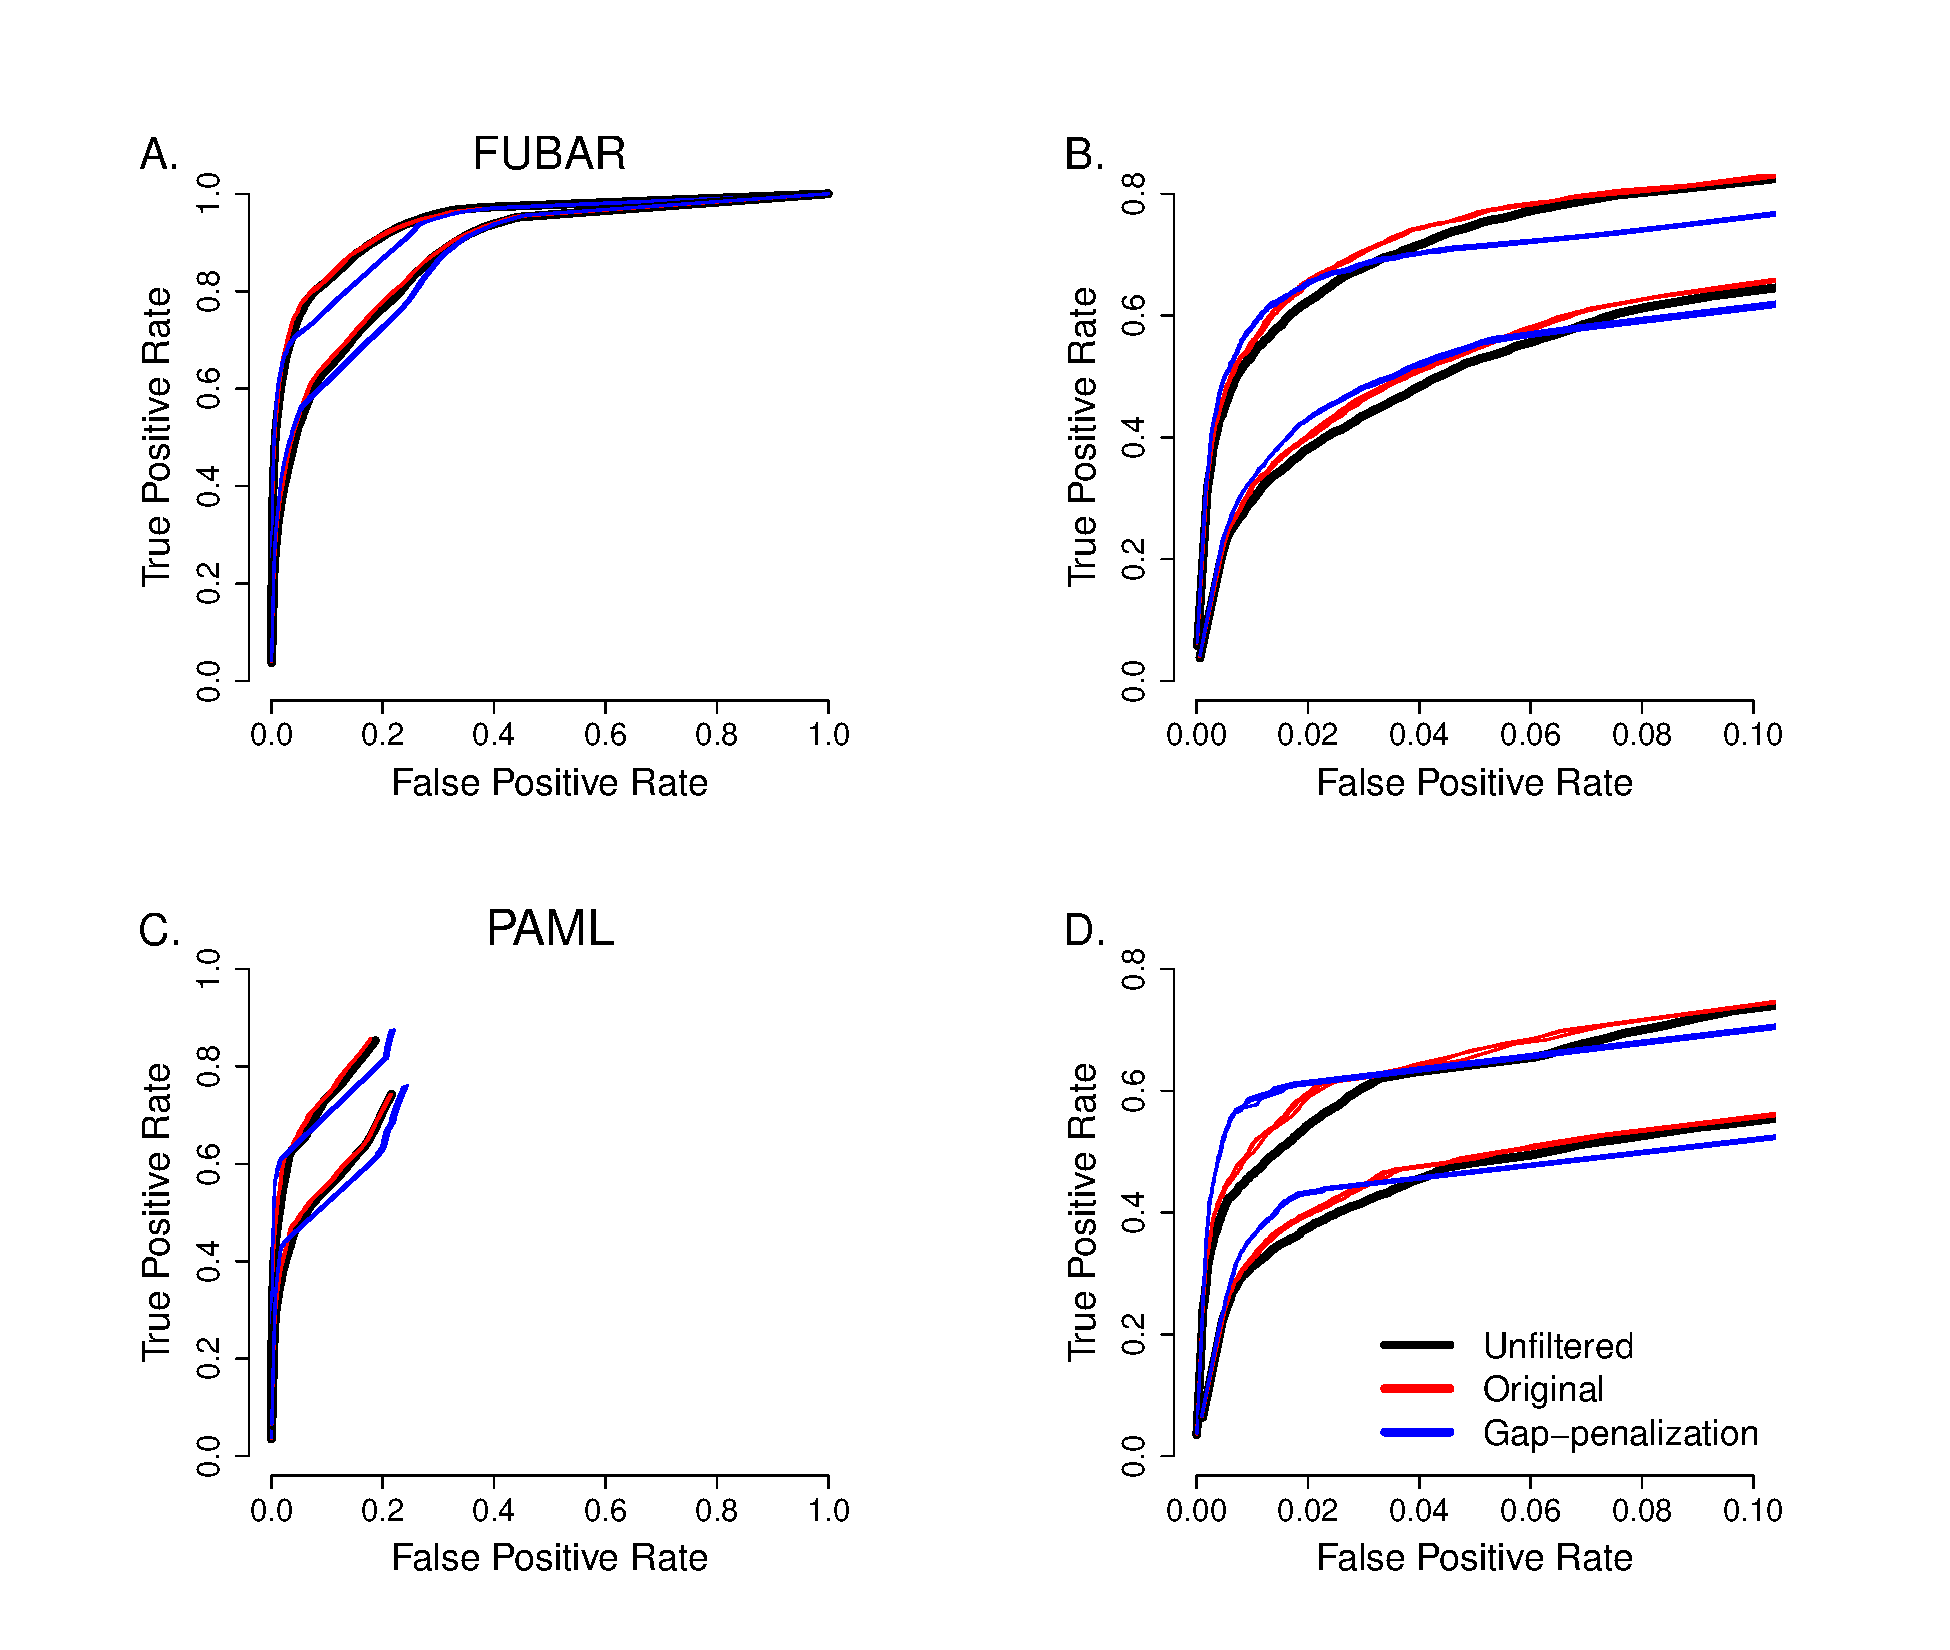
\includegraphics[width=6in]{Figures/ROC_prk.pdf}}
\caption{\label{roc} ROC curves as averaged across the two 60 sequence simulation sets. For all panels, the top curve represents results from the HA selective profile, and the bottom curve represents results from the GP41 selective profile. A-B) ROC curves for positive-selection inference by FUBAR. C-D) ROC curves for positive-selection inference by PAML M8.}
\end{figure*}

%\bigskip



%%%%%%%%%%%%%%%%%%%%%%%%%%%%%%%%%%%%%%%%%%%%%%%%%%%%%%%%%%%%%%%%%%%%%%%%%%%%%%%%%%%%%%%%%%%%%%%%%%%%%%%%%%%%%%%%%%%%%%%%%%%%%%%%%%%%%%%%%%%%%%%%%%%%%%%%%%%%%%%%%%%%%%%%
\begin{table}[htbp]
\begin{adjustwidth}{-1.85cm}{}
\caption {\label{tab:summarystats} Summary statistics for effect of masking.}
\begin{tabular}{l l l l l l l}
\hline\noalign{\smallskip}
& & & \multicolumn{4}{c}{Mean True Positive Rate} \\
\cline{4-7}\noalign{\smallskip}
\multicolumn{1}{c}{Selective Profile} & \multicolumn{1}{c}{Number of Taxa} & \multicolumn{1}{c}{Inference Method} & \multicolumn{1}{l}{True} & \multicolumn{1}{l}{Unfiltered} & \multicolumn{1}{l}{Guidance} & \multicolumn{1}{l}{GuidanceP} \\
\noalign{\smallskip}\hline\noalign{\smallskip}
HA  &  11  &  FUBAR  &  0.093  &  0.084  &  0.085 (1.33\%)  &  0.085 (0.74\%) \\
  &    &  PAML  &  0.086  &  0.082  &  0.081 (-0.48\%)  &  0.081 (-0.60\%)\\
\hline
 & 26 & FUBAR & 0.252 & 0.227 & 0.229 (0.84\%) & 0.226 (-0.38\%) \\
 &   & PAML & 0.209 & 0.176 & \textbf{0.178 (1.36\%)$^{\ast\ast}$} & \textbf{0.183 (4.04\%)$^{\ast\ast}$} \\
\hline
 & 60 & FUBAR & 0.551 & 0.474 & 0.479 (0.99\%) & \textbf{0.464 (-2.16\%)$^{\ast}$}  \\
 &  & PAML & 0.422 & 0.347 & 0.342 (-1.68\%) & 0.337 (-2.92\%) \\
 \hline
 & 158 & FUBAR & 0.515 & 0.458 & \textbf{0.467 (1.89\%)$^{\ast}$} & \textbf{0.468 (2.12\%)$^{\ast}$} \\
\hline
GP41  &  11 &  FUBAR  &  0.062  &  0.058  &  0.057 (-1.55\%)  &  0.057 (-1.21\%)\\
  &    &  PAML  &  0.096  &  0.098  &  \textbf{0.095 (-3.49\%)$^{\ast\ast}$}  &  \textbf{0.095 (-3.80\%)$^{\ast\ast}$} \\
\hline
 & 26 & FUBAR & 0.216 & 0.196 & \textbf{0.20 (1.89\%)$^{\ast}$} & 0.197 (0.36\%) \\
 & & PAML & 0.237 & 0.216 & 0.220 (1.54\%) & 0.217 (0.244\%) \\
 \hline
 & 60 & FUBAR & 0.359 & 0.308 & \textbf{0.313 (1.77\%)$^{\ast}$} & 0.304 (-1.16\%)\\
 & & PAML & 0.341 & 0.304 & 0.302 (-0.77\%) & \textbf{0.296 (-2.71\%)$^{\ast\ast}$} \\
 \hline
 & 158 & FUBAR & 0.348 & 0.320 & \textbf{0.325 (1.77\%)$^{\ast\ast}$} & \textbf{0.326 (2.02\%)$^{\ast\ast}$} \\
 \hline
\end{tabular}
\newline
\textsc{note.}--- Significance levels:  $^{\ast\ast} P < 0.001$; $^{\ast} P < 0.01$. Mean TPR values shown in bold represent those which are significantly different from the respective unfiltered MSA mean TPR. Values shown in parentheses refer to the average TPR percent change from the respective unfiltered MSA. All significance levels were corrected for multiple comparisons using the R multcomp package \citep{Hothorn2008}.
\end{adjustwidth}
\end{table}
%%%%%%%%%%%%%%%%%%%%%%%%%%%%%%%%%%%%%%%%%%%%%%%%%%%%%%%%%%%%%%%%%%%%%%%%%%%%%%%%%%%%%%%%%%%%%%%%%%%%%%%%%%%%%%%%%%%%%%%%%%%%%%%%%%%%%%%%%%%%%%%%%%%%%%%%%%%%%%%%%%%%%%%%







\end{document}